\section{Задача 2.2}
\subsection{Задание:}
Вычислить
$
	\dfrac{(1+i)^9}{(1-i)^9}
$
\subsection{Решение:}
$
	\dfrac{(1+i)^9}{(1-i)^9}
	=
	(\dfrac{(1+i)}{(1-i)})^9
	=
	(\dfrac{(1+i)(1+i)}{(1+i)(1-i)})^9
	=
	(\dfrac{1 - 2i - 1}{1 + 1})^9
	=
	\\[1em]
	=
	(-i)^{25}
	=
	(-i)^{24} \cdot i
	=
	(-1)^{12} \cdot i
	=
	1 \cdot i
	=
	i
$
\subsection{Компьютерная проверка в среде Wolfram Mathematica}
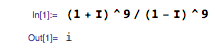
\includegraphics[scale=0.6]{task/2_02/screen1.png}
\subsection{Вывод:}
Мы правильно вычислили значение выражения.
